\chapter{Simulations of DTU 10~MW RWT}

Figure~\ref{f:4ms}~--~\ref{f:24ms} shows selected signals from IEC NTM simulations with HAWC2 of the class 1A DTU 10~MW RWT at 4, 8, 12, 16, 20, and 24~m/s. All simulations are only meant as an example of the controller performance because they are performed using an earlier version of the DTU 10~MW RWT than the published one. The plots include the initial transients. Comments to simulations are given in the captions.


\begin{figure}[t]
\centerline{\epsfig{figure=sim4ms.eps,width=0.99\textwidth} }
\caption{Selected signals from IEC NTM simulation of the class 1A DTU 10~MW RWT at 4~m/s. Note the long start-up time (transients) which for low wind speeds can be reduced by setting a higher initial rotor speed. Note also that a minimum pitch angle varies and that the integral pitch term is positive. \label{f:4ms}}
\end{figure}


\begin{figure}[t]
\centerline{\epsfig{figure=sim8ms.eps,width=0.99\textwidth} }
\caption{Selected signals from IEC NTM simulation of the class 1A DTU 10~MW RWT at 8~m/s. Note the generator is mainly running at its minimum speed. As the speed increases, the speed set point switches at the speed crosses the averaged between rated and this minimum speed, which causes the discontinuities on the torque limits. The variation of minimum pitch angle with wind speed is also seen. The integral pitch term is still positive. \label{f:8ms}}
\end{figure}


\begin{figure}[t]
\centerline{\epsfig{figure=sim12ms.eps,width=0.99\textwidth} }
\caption{Selected signals from IEC NTM simulation of the class 1A DTU 10~MW RWT at 12~m/s. At this close to rated wind speeds, the turbine is starting to produce full power. During the transients, the pitch controller controls the rotor speed and the larger-than-minimum pitch results in a switch value of 1, whereby the torque reference is set to constant power control. Around 200~s, the wind speed has lowered, resulting in a lowering rotational speed, the pitch controller lowers the pitch angle, and eventually the switch goes to zero, i.e., partial load operation. \label{f:12ms}}
\end{figure}


\begin{figure}[t]
\centerline{\epsfig{figure=sim16ms.eps,width=0.99\textwidth} }
\caption{Selected signals from IEC NTM simulation of the class 1A DTU 10~MW RWT at 16~m/s. The turbine stays in full load operation. \label{f:16ms}}
\end{figure}


\begin{figure}[t]
\centerline{\epsfig{figure=sim20ms.eps,width=0.99\textwidth} }
\caption{Selected signals from IEC NTM simulation of the class 1A DTU 10~MW RWT at 20~m/s. The turbine stays in full load operation. \label{f:20ms}}
\end{figure}


\begin{figure}[t]
\centerline{\epsfig{figure=sim24ms.eps,width=0.99\textwidth} }
\caption{Selected signals from IEC NTM simulation of the class 1A DTU 10~MW RWT at 24~m/s. The turbine stays in full load operation. \label{f:24ms}}
\end{figure}


\begin{figure}[!t]
\begin{center}
\parbox{0.9\columnwidth}{\mbox{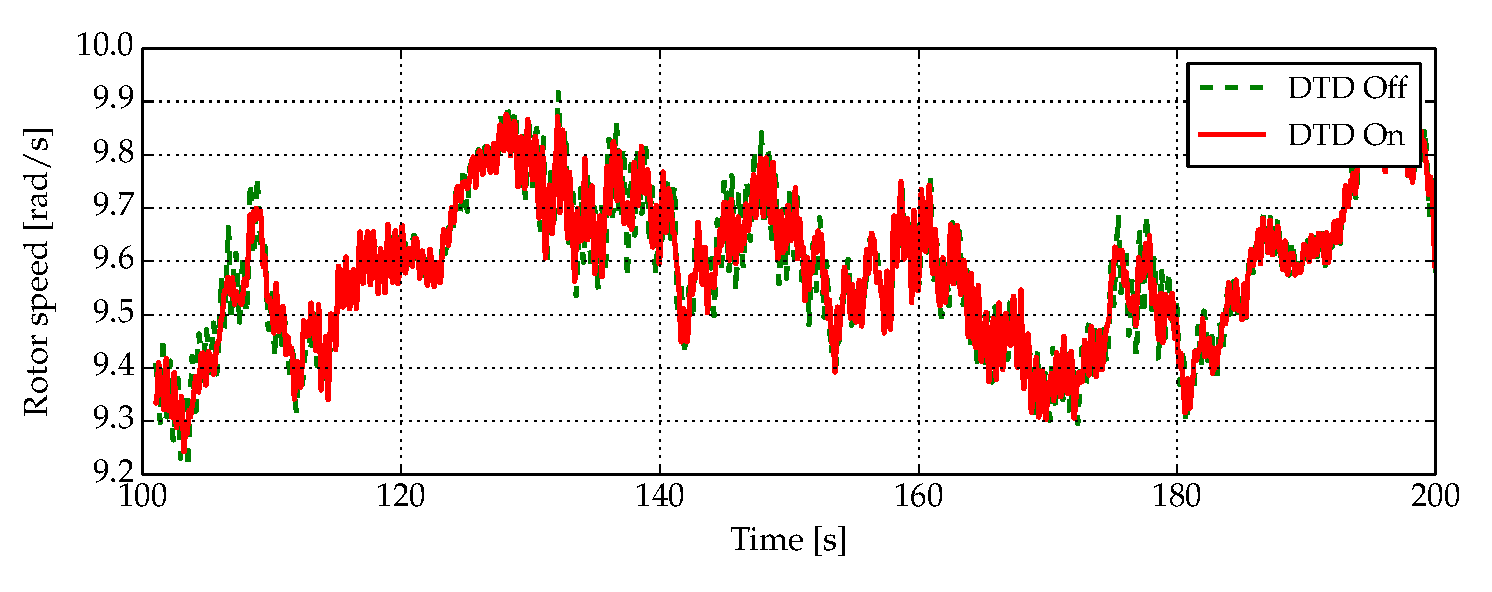
\includegraphics[keepaspectratio=true,width=0.9\columnwidth]{DTD_rotorspeed}}}\\
\parbox{0.9\columnwidth}{\mbox{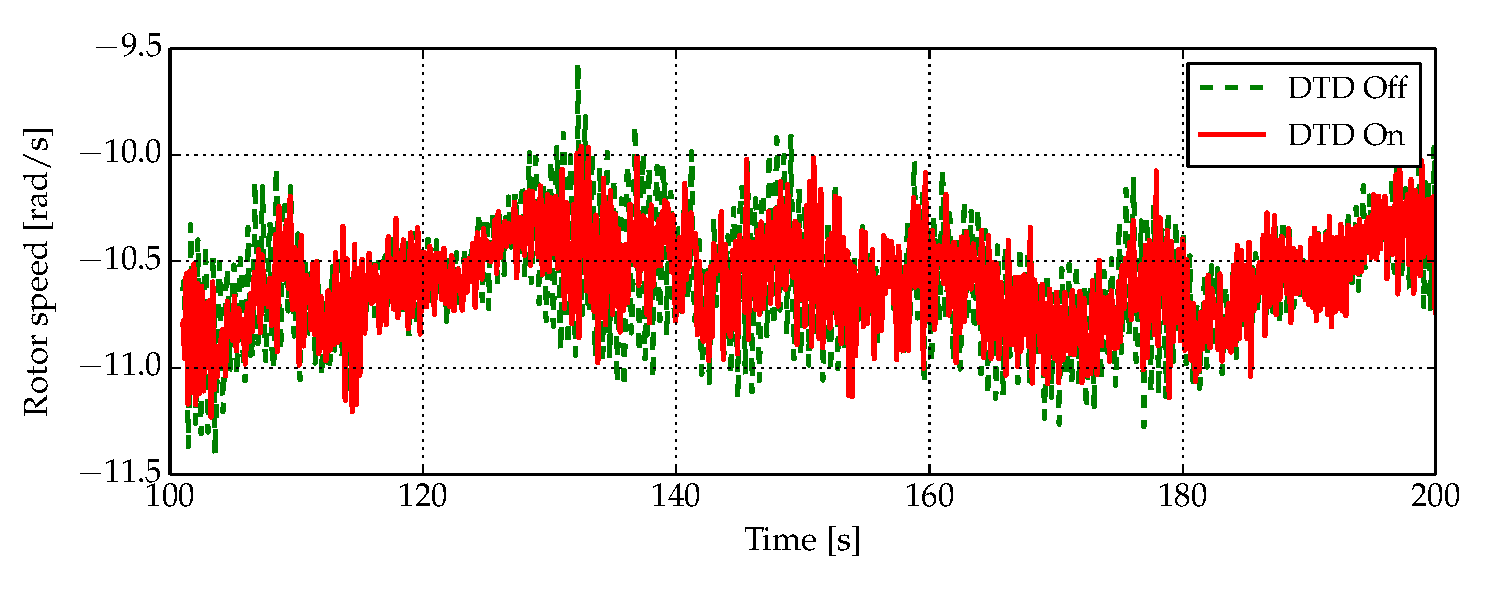
\includegraphics[keepaspectratio=true,width=0.9\columnwidth]{DTD_torque}}}\\
\parbox{0.9\columnwidth}{\mbox{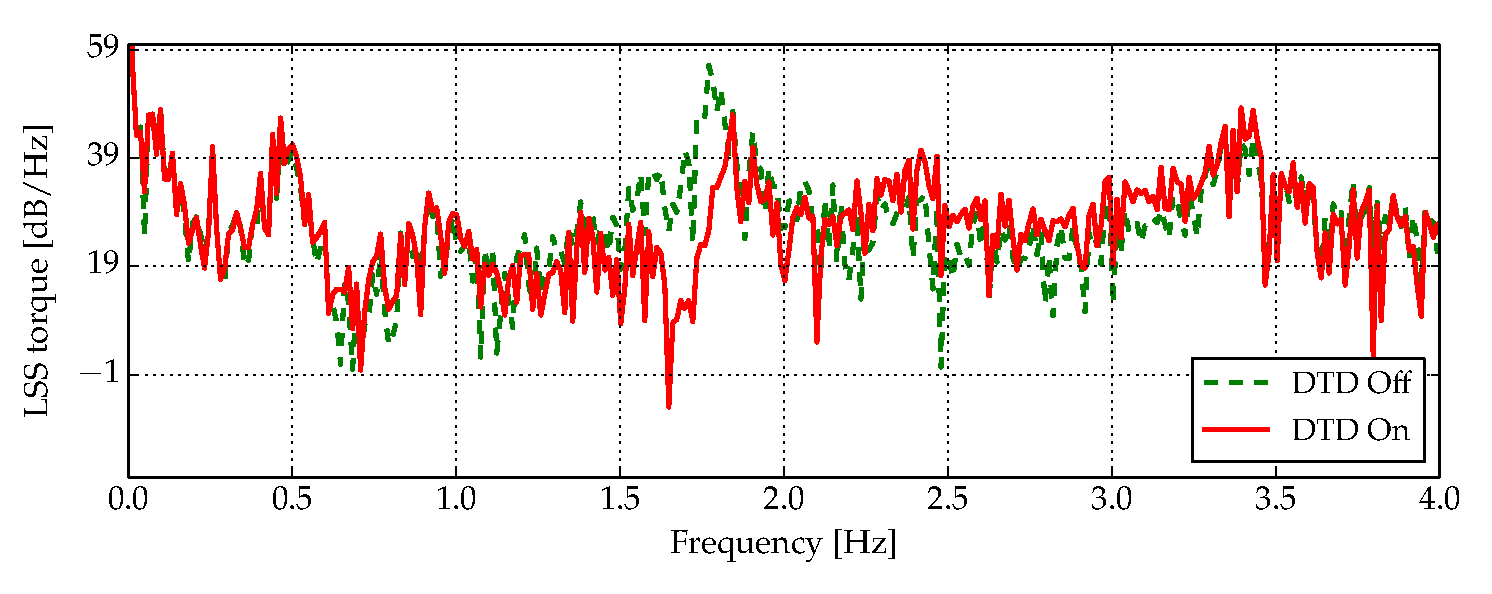
\includegraphics[keepaspectratio=true,width=0.9\columnwidth]{DTD_torque_psd}}}
\caption{Drivetrain damper. Rotor speed time series and LSS torque time series and power spectral density. Wind speed 12 m/s and turbulence intensity of 20\%.}\label{f:DT_damper}
\end{center}
\end{figure}

\begin{figure}[t]
\begin{center}
\parbox{0.9\columnwidth}{\mbox{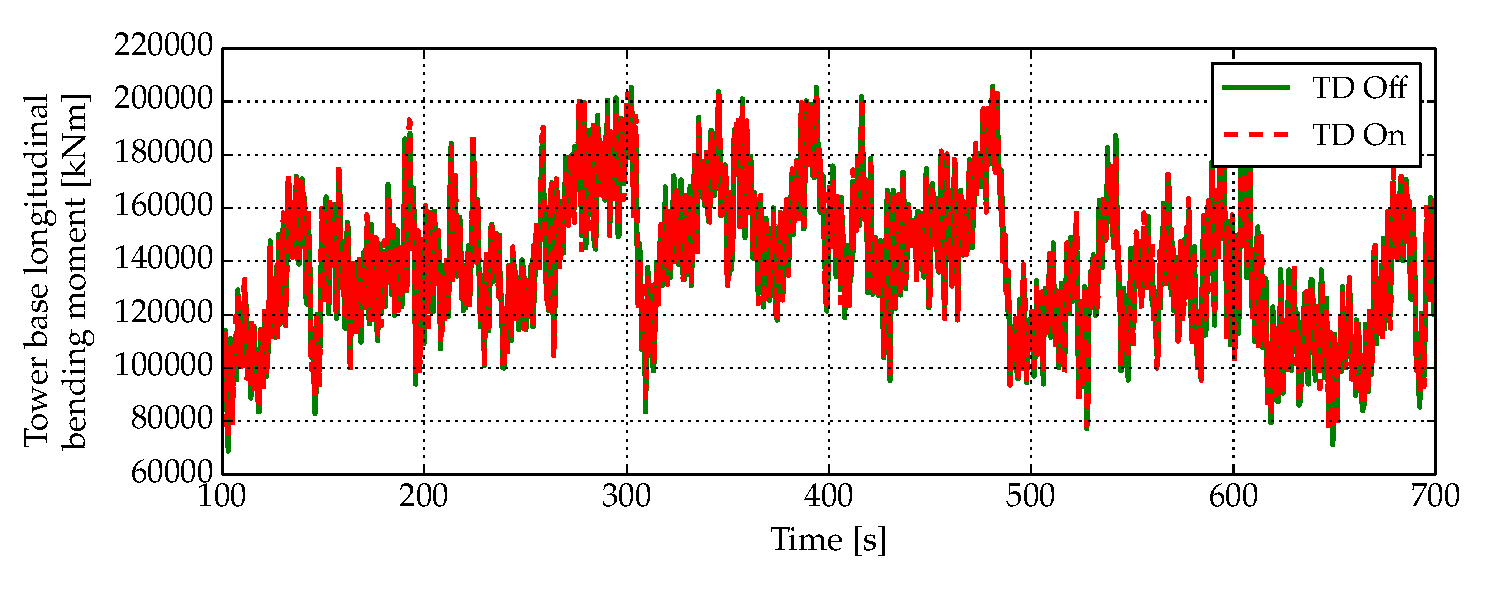
\includegraphics[keepaspectratio=true,width=0.9\columnwidth]{TD_tower}}}\\
\parbox{0.9\columnwidth}{\mbox{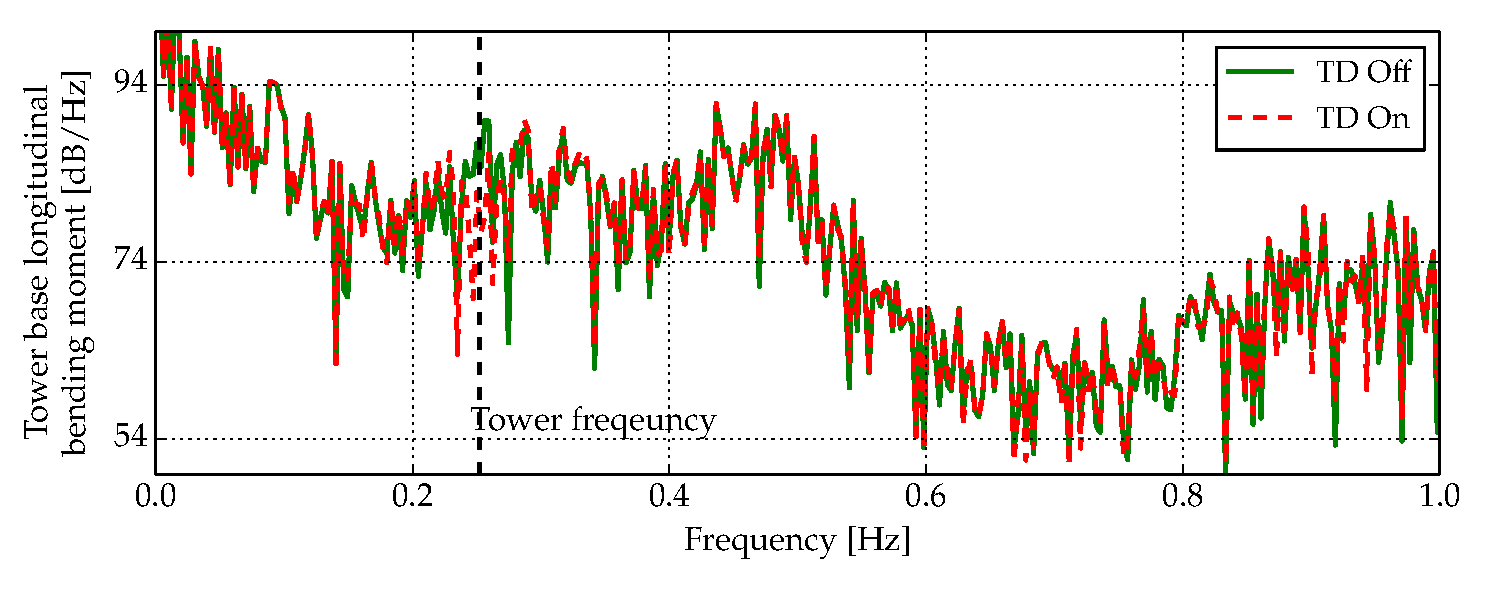
\includegraphics[keepaspectratio=true,width=0.9\columnwidth]{TD_tower_psd}}}
\caption{Longitudinal tower damper. Longitudinal tower base bending moment time series and power spectral density. Wind speed 12 m/s and turbulence intensity of 20\%.}\label{f:TT_damper}
\end{center}
\end{figure}

\begin{figure}[!t]
\begin{center}
\parbox{0.9\columnwidth}{\mbox{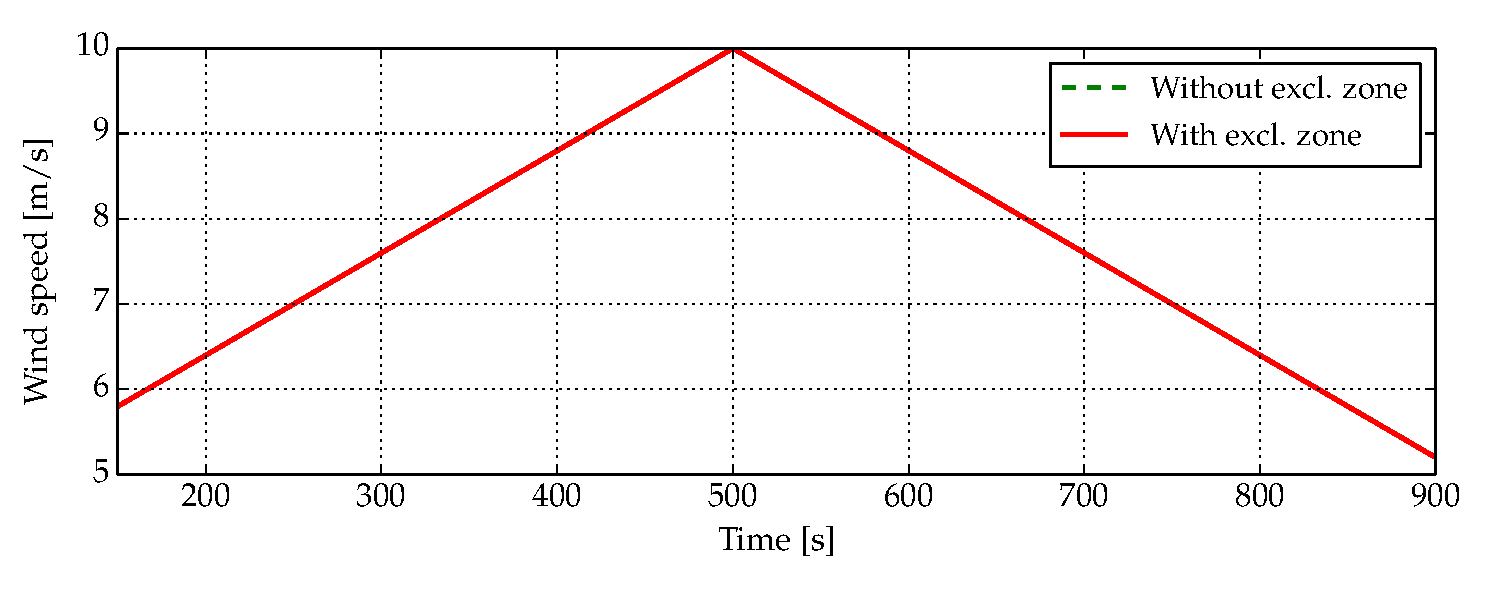
\includegraphics[keepaspectratio=true,width=0.9\columnwidth]{EZ_windspeed}}}\\
\parbox{0.9\columnwidth}{\mbox{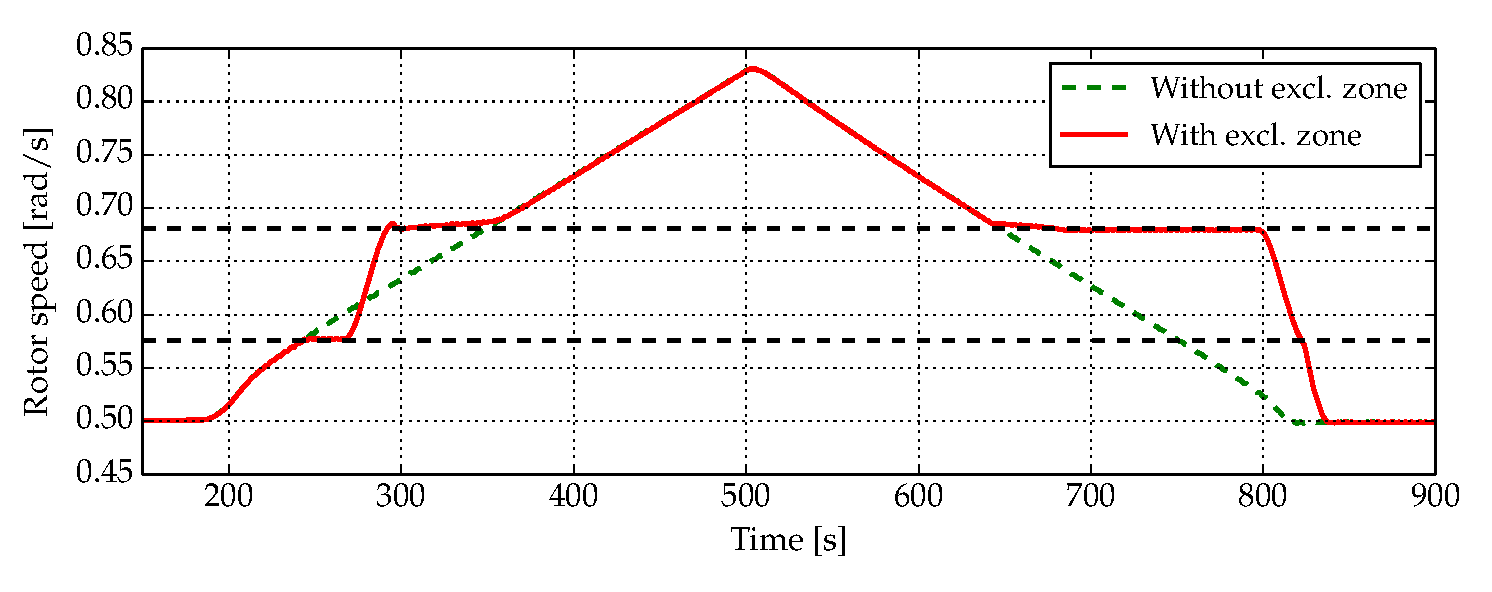
\includegraphics[keepaspectratio=true,width=0.9\columnwidth]{EZ_rotorspeed}}}\\
\parbox{0.9\columnwidth}{\mbox{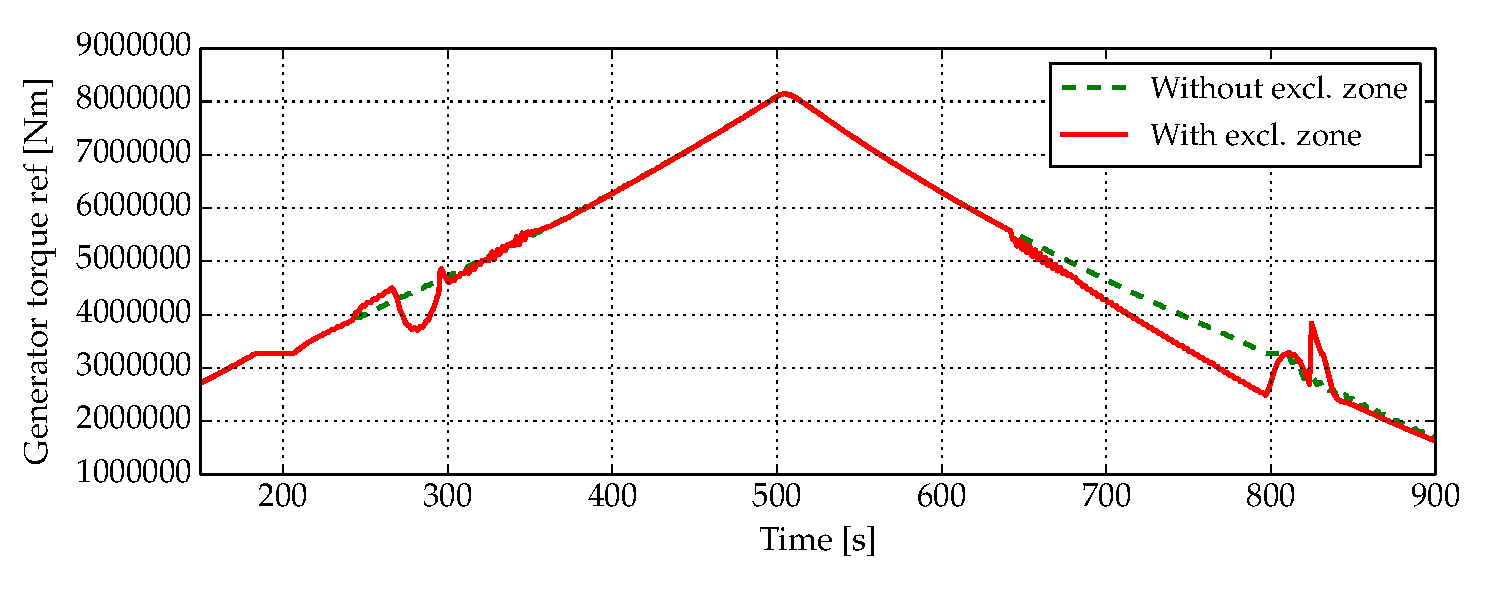
\includegraphics[keepaspectratio=true,width=0.9\columnwidth]{EZ_torque}}}
\caption{Exclusion zone. Wind speed, rotor speed, and LSS torque.}\label{f:EZ}
\end{center}
\end{figure}

\begin{figure}[!t]
\begin{center}
\parbox{0.9\columnwidth}{\mbox{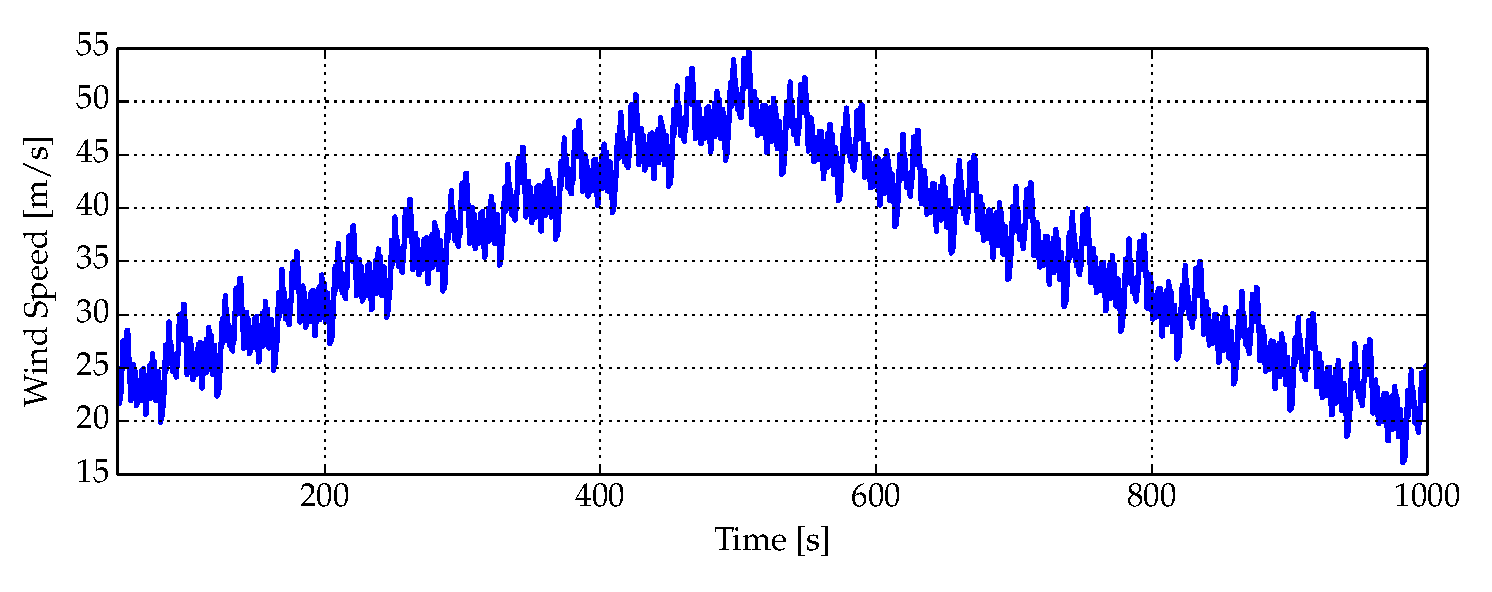
\includegraphics[keepaspectratio=true,width=0.9\columnwidth]{Storm_windspeed}}}\\
\parbox{0.9\columnwidth}{\mbox{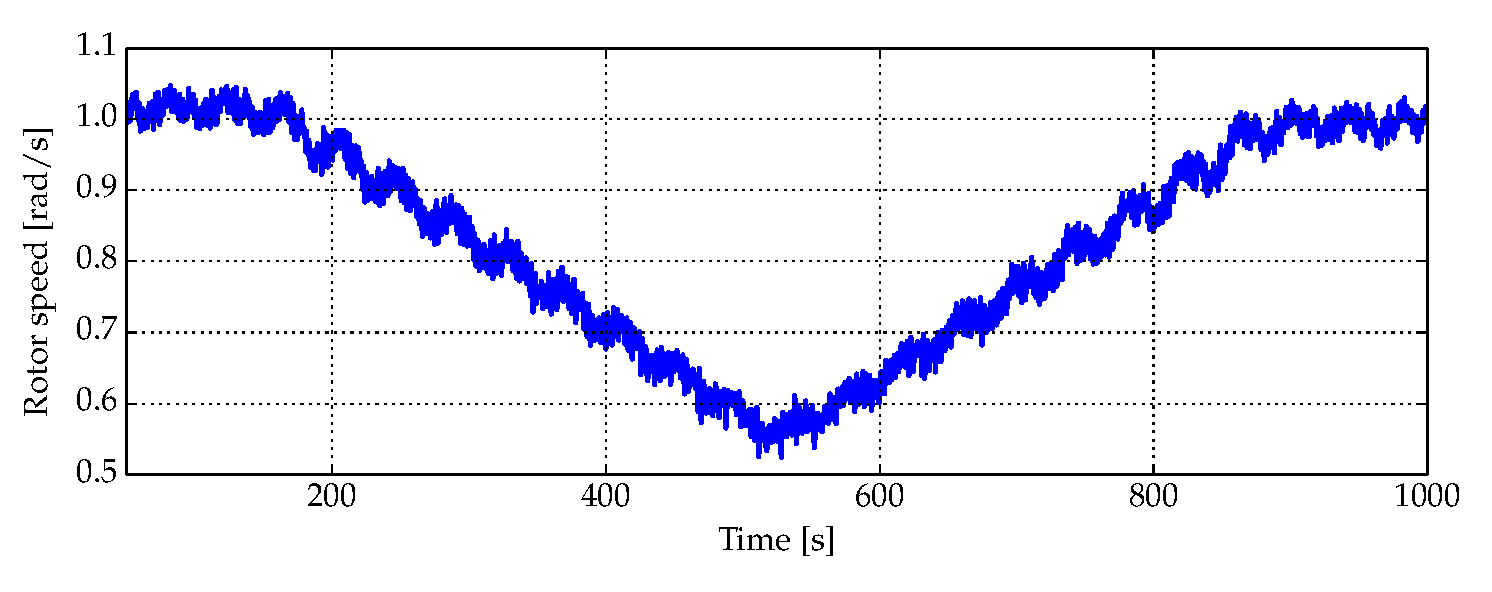
\includegraphics[keepaspectratio=true,width=0.9\columnwidth]{Storm_rotorspeed}}}\\
\parbox{0.9\columnwidth}{\mbox{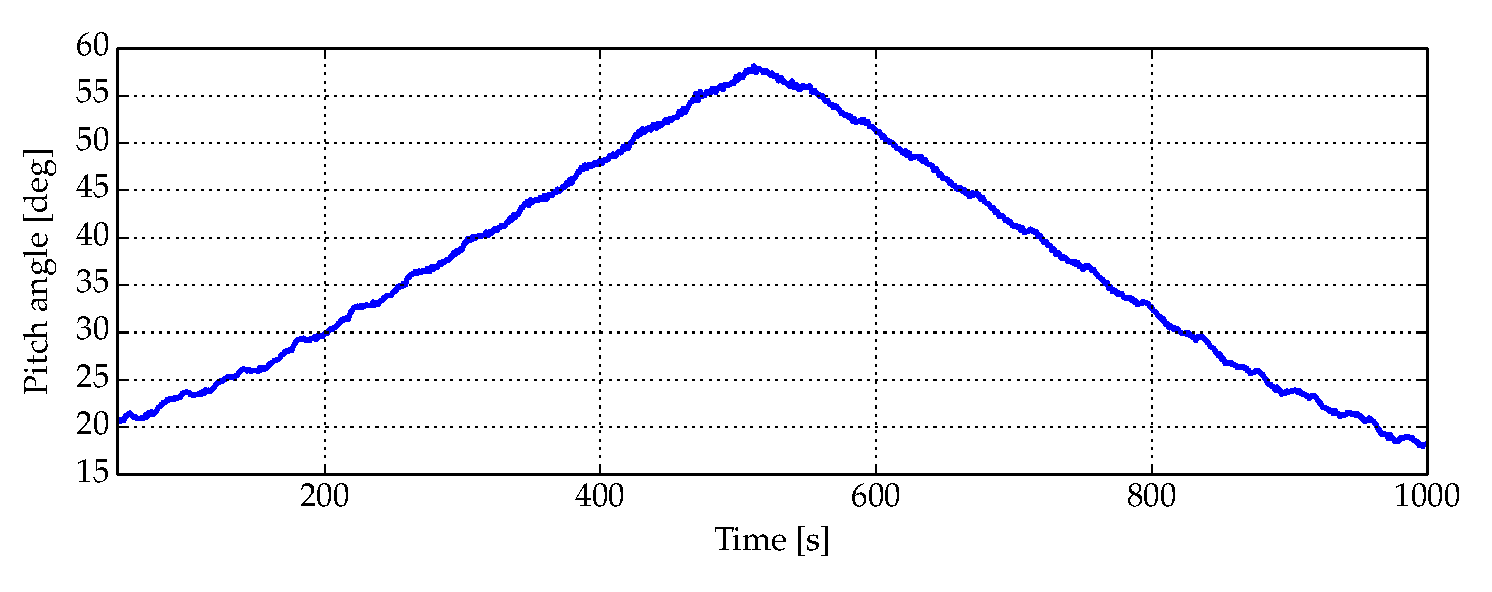
\includegraphics[keepaspectratio=true,width=0.9\columnwidth]{Storm_pitch}}}
\caption{Storm control. Wind speed, rotor speed, and pitch angle.}\label{f:StormControl}
\end{center}
\end{figure}